\chapter{Implementazione}
\label{chap:implementazione}
In questo capitolo si mostra come sono state implementate le funzionalità richieste dalle user stories mostrate nella tabella \ref{tab:user:sto}.
Per ogni funzionalità vedremo quali API sono state create, come sono state documentate attraverso Postman ed il codice utilizzato per realizzarle.

Tutte le rotte relative ai servizi API sono presenti nel file \texttt{/routes.js}, ad esclusione dei servizi relativi alla registrazione e autenticazione di un utente, che si trovano direttamente nel file \texttt{/app.js}.
\section{US-01/03}
Per l'implementazione delle prime tre user stories, che verrano trattate insieme, essendo per lo più simili tra loro, sono stati creati i seguenti servizi:
\begin{lstlisting}[{caption=/routes.js}, style=JavaScriptCode]
module.exports = function(app){
	var List = require('./controllers/lists');
	var Object = require('./controllers/objects');
	var Part = require('./controllers/parts');
	var Option = require('./controllers/options');
	
	app.get('/lists', List.findAll);
	app.get('/lists/:id', List.findById);
	app.post('/lists', List.add);
	app.put('/lists/:id', List.update);
	app.delete('/lists/:id', List.delete);
	
	app.get('/objects/:listid', Object.findAll);
	app.get('/objects/:id', Object.findById);
	app.post('/objects/:listid', Object.add);
	app.put('/objects/:id', Object.update);
	app.delete('/objects/:id', Object.delete);
	
	app.get('/parts/:objectid', Part.findAll);
	app.get('/parts/:id', Part.findById);
	app.post('/parts/:objectid', Part.add);
	app.put('/parts/:id', Part.update);
	app.delete('/parts/:id', Part.delete);
	
	app.get('/options/:partid', Option.findAll);
	app.get('/options/:id', Option.findById);
	app.post('/options/:partid', Option.add);
	app.put('/options/:id', Option.update);
	app.delete('/options/:id', Option.delete);
}
\end{lstlisting}
Come si può vedere, ad ogni operazione CRUD è associata la relativa API, che esegue una specifica funzione presente nel file corrispondente. I file relativi alle suddette funzioni sono contenuti nella cartella \texttt{controllers} e vengono richiamati all'inizio del file \texttt{routes.js}.

Le funzioni sono sufficientemente autoesplicative, ma per chiarezza vengono elencate ed esposte qui di seguito:
\begin{itemize}
	\item \texttt{app.get} si divide in due casi:
	\begin{enumerate}
		\item \texttt{/API} in cui vengono richiesti tutti i Document di una Collection. Nel caso in cui la Collection sia un Object, una Option o una Part, viene passato in input il parametro \texttt{:id} che identifica il Document \emph{parente}.
		\item \texttt{/API/:id} in cui viene passato il parametro \texttt{:id}, per interrogare la Collection nel database MongoDB secondo il criterio di identificazione.
	\end{enumerate}
	\item \texttt{app.post} \\Con questa operazione si aggiunge un Document alla corrispondente Collection. Questo è l'unico caso in cui vanno distinte le Lists dagli altri oggetti. Quando si aggiunge una List tramite metodo POST, non viene passato nessun parametro alla chiamata API. Si noti invece che negli altri casi, durante la medesima operazione, viene sempre passato l'id dell'oggetto \emph{parente}, dell'oggetto ossia a cui fa riferimento il Document che stiamo inserendo.
	\item \texttt{app.put} \\Questa operazione viene usata per modificare un Document già presente in una Collection. Prende in input il parametro \texttt{:id} per poter ritrovare il giusto oggetto su cui eseguire un \emph{update}.
	\item \texttt{app.delete} \\Infine l'operazione \emph{delete} si usa per eliminare un Document specifico, che viene identificato, come sopra, prendendo in input il parametro \texttt{:id}. 
\end{itemize}

Di seguito prendiamo in esame il controller relativo agli Objects per analizzare le relative funzioni, seguite dalla relativa documentazione realizzata con Postman:
\begin{lstlisting}[{caption=/controllers/objects.js}, style=JavaScriptCode]
var mongoose = require('mongoose'),
Object = require('../app/schema.js').model('Object');

exports.findAll = function(req, res){
	var listid = req.params.listid;
	Object.find({'_list': listid},function(err, docs) {
		return res.send(docs);
	});
};

exports.findById = function(req, res){
	var id = req.params.id;
	Object.findOne({'_id': id, '_list': listid},function(err, docs) {
		return res.send(docs);
	});
};

exports.add = function(req, res) {
	var listid = req.params.listid;
	Object.create({"nome": req.body.nome, "descrizione": req.body.descrizione, 
	"_list": listid}, function (err, docs) {
		if (err) return console.log(err);
		return res.send(docs);
	});
};

exports.update = function(req, res) {
	var id = req.params.id;
	var updates = req.body;
	console.log(id);
	Object.update({"_id":id}, req.body,
	function (err, numberAffected) {
		if (err) return console.log(err);
		console.log('Updated %d Lists', numberAffected);
		return res.sendStatus(202);
	});
};

exports.delete = function(req, res) {
	var id = req.params.id;
	Object.remove({'_id':id},function(result) {
		return res.send(result);
	});
};
\end{lstlisting}

L'interfacciamento con il database è gestito tramite mongoose, di cui viene importata la dipendenza all'inizio del file.
La prima funzione è \texttt{findAll}, che prende in input, attraverso i parametri presenti nella request, l'id della List a cui l'Object è associato. Viene quindi eseguita la funzione \texttt{.find} di mongoose sulla Collection Objects, filtrando per l'id appena passato, e quello che si avrà come risposta sarà una callback, che conterrà un messaggio di errore in caso di fallimento, o i Document richiesti in caso di successo. A questo punto il server invia la risposta tramite la funzione \texttt{res.send}, includendo i risultati dell'interrogazione appena effettuata sul database. La funzione \texttt{findById} è molto simile alla precedente, pertanto non verrà spiegata nuovamente.
\begin{figure}[h]
	\centering
	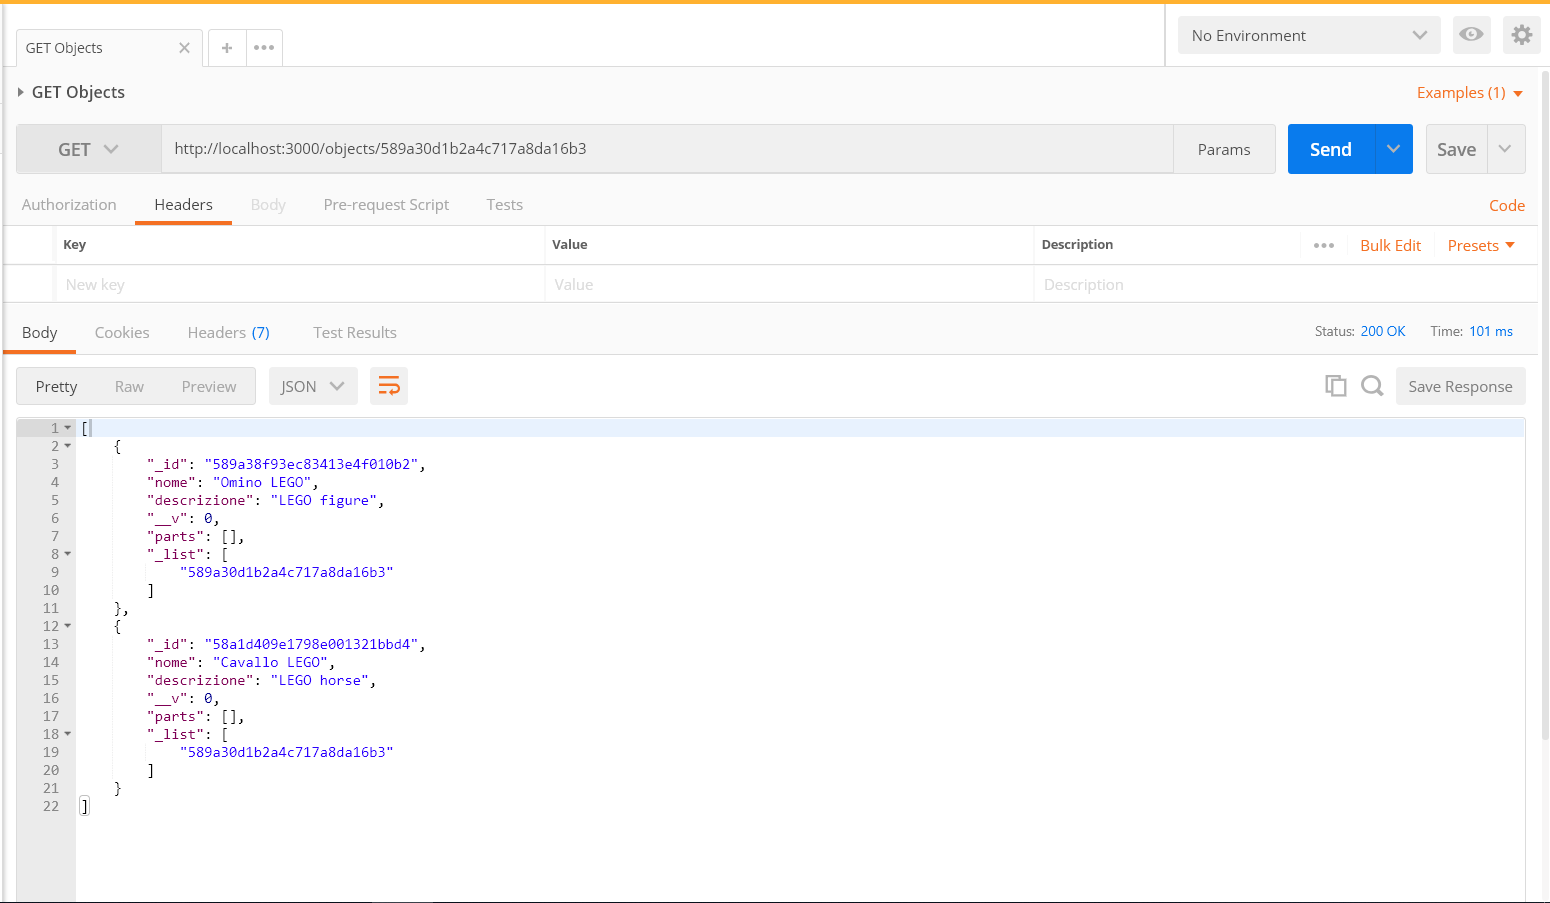
\includegraphics[scale=0.42]{Immagini/get_objects.png}
	\caption{Documentazione get /objects/:id}
\end{figure}

La funzione \texttt{add} inserisce un nuovo Object Document nella sua Collection, solo dopo però averlo inizializzato inserendo l'id della List a cui fa riferimento nell'attributo \texttt{\_list}, il nome (preso dal \emph{body} della richiesta HTTP) nell'attributo \texttt{nome} e la descrizione nel corrispondente attributo. I parametri nome e descrizione sono stati inseriti dall'utente negli appositi campi presenti nella pagina di visualizzazione degli Objects, e vengono trasmessi al server attraverso la richiesta HTTP POST.
\begin{figure}[h]
	\centering
	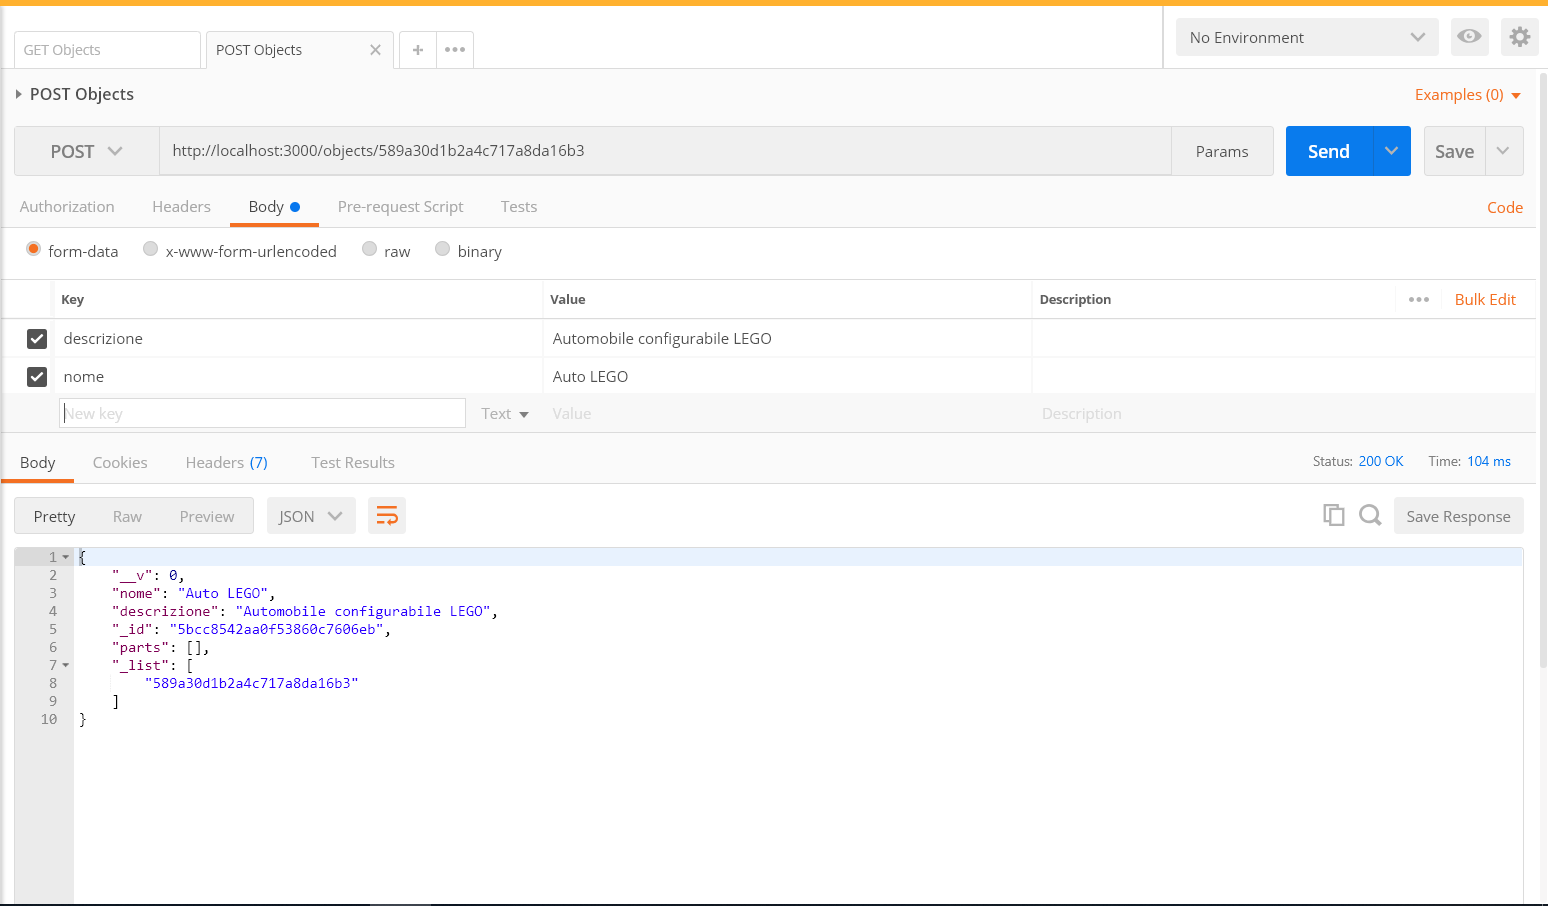
\includegraphics[scale=0.42]{Immagini/post_objects.png}
	\caption{Documentazione post /objects/:id}
\end{figure}

L'ultima funzione è \texttt{delete}. Questa rimuove l'Object cercandolo attraverso il suo \texttt{id}. La funzione non necessita di alcun parametro aggiuntivo.
\begin{figure}[h]
	\centering
	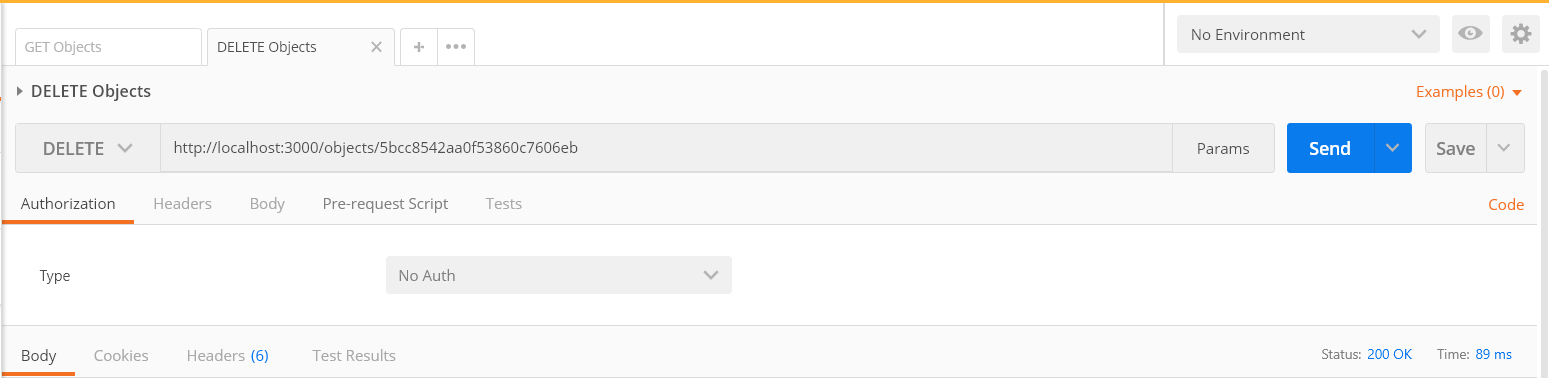
\includegraphics[scale=0.42]{Immagini/delete_objects.png}
	\caption{Documentazione delete /objects/:id}
\end{figure}

Le funzioni si comportano in modo analogo, o comunque come spiegato sopra, con gli altri tipi di oggetti in unicam-product-editor.
Per quanto riguarda la funzione di visualizzazione dei documenti richiesta dalle user stories dalla 01 alla 03, è stata sviluppata una applicazione single-page in AngularJS, che andremo a vedere nella US-05.
\section{US-04}
La user story 04 richiede di avere un endpoint che restituisca la forma JSON di un oggetto 3D da visualizzare.

Per implementare questa funzione, è stata creata una chiamata API apposita, contenuta nel file del server \texttt{app.js}.

\begin{lstlisting}[{caption=shape API}, style=JavaScriptCode]
app.get('/shape/:id', cors(corsOptions), function(req, res){
	var search = req.params.id;
	converted(req, search, res);
});
\end{lstlisting}
Come possiamo vedere dallo snippet di codice qui sopra, la API rimanda alla apposita funzione converted, situata in \texttt{/app/converted.js}.

\begin{lstlisting}[{caption=/app/converted.js}, style=JavaScriptCode]
coll.find({"_id" : mongodb.ObjectId(search)}).toArray(function(err, docs) {
	if (err){
		console.log('error in db');
		res.end();
		return;
	}
	else if (docs.length == '0'){
		console.log('No files found');
		res.send('No files found');
	}
	else{
		res.send(docs);
	}
});
\end{lstlisting}
Lo scopo della funzione è quello di trovare nella Collection Shapes il documento JSON corrispondente a quello dell'id richiesto. In questa particolare Collection, i JSON non seguono uno Schema come nel caso degli altri oggetti, ma vengono conservati così come sono, essendo questi il risultato della conversione dei file .obj. Così quando il server risponderà, non lo farà usando uno stato risultante di una richiesta HTTP, ma lo farà inviando il JSON vero e proprio. Grazie a questo tipo di risposta, unicam-product-viewer avrà il suo enpoint a cui agganciarsi per prendere le forme 3D da visualizzare nella propria interfaccia.
\begin{figure}[h]
	\centering
	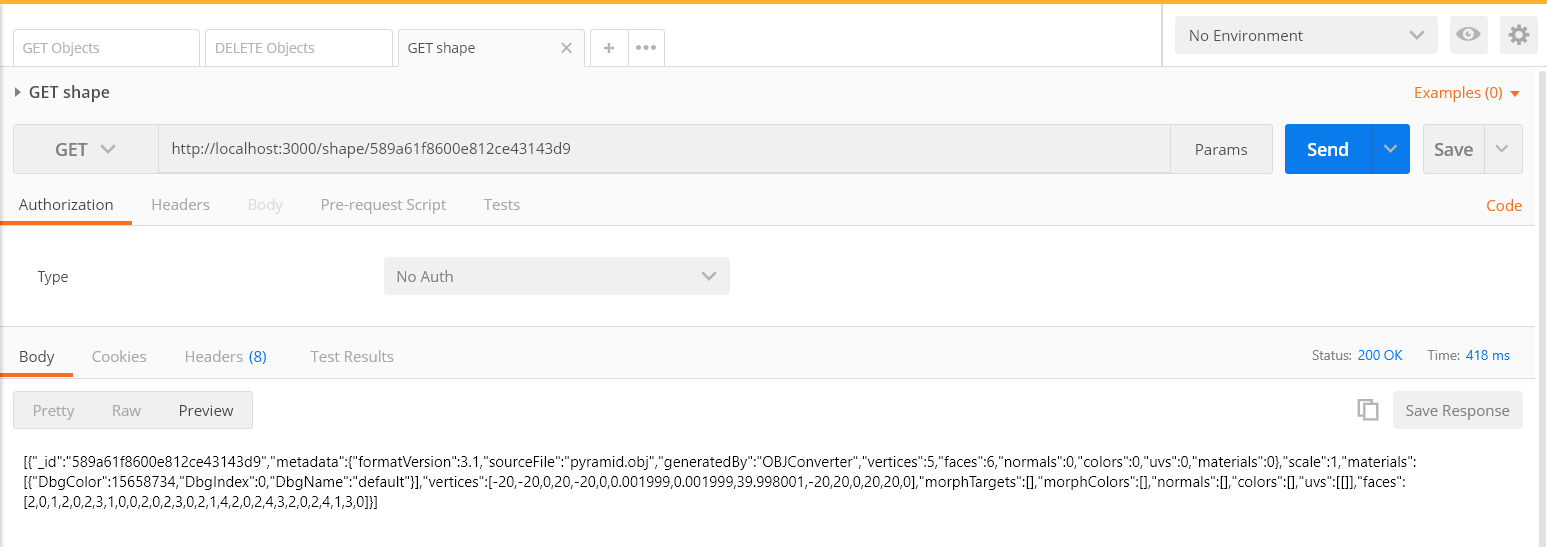
\includegraphics[scale=0.42]{Immagini/get_shape.png}
	\caption{Documentazione get /shape/:id}
\end{figure}
